% !TEX encoding = UTF-8 Unicode
% REMEMBER TO SET LANGUAGE!
\documentclass[a4paper,10pt,norsk]{article}
\usepackage[utf8]{inputenc}
\usepackage[norsk]{babel}
% Standard stuff
\usepackage{amsmath,graphicx,varioref,verbatim,amsfonts,geometry}
% colors in text
\usepackage[usenames,dvipsnames,svgnames,table]{xcolor}
% Hyper refs
\usepackage[colorlinks]{hyperref}

% Document formatting
\setlength{\parindent}{0mm}
\setlength{\parskip}{1.5mm}

%Color scheme for listings
\usepackage{textcomp}
\definecolor{listinggray}{gray}{0.9}
\definecolor{lbcolor}{rgb}{0.9,0.9,0.9}

%Listings configuration
\usepackage{listings}
%Hvis du bruker noe annet enn python, endre det her for å få riktig highlighting.
\lstset{
	backgroundcolor=\color{lbcolor},
	tabsize=4,
	rulecolor=,
	language=python,
        basicstyle=\scriptsize,
        upquote=true,
        aboveskip={1.5\baselineskip},
        columns=fixed,
	numbers=left,
        showstringspaces=false,
        extendedchars=true,
        breaklines=true,
        prebreak = \raisebox{0ex}[0ex][0ex]{\ensuremath{\hookleftarrow}},
        frame=single,
        showtabs=false,
        showspaces=false,
        showstringspaces=false,
        identifierstyle=\ttfamily,
        keywordstyle=\color[rgb]{0,0,1},
        commentstyle=\color[rgb]{0.133,0.545,0.133},
        stringstyle=\color[rgb]{0.627,0.126,0.941}
        }
        
\newcounter{subproject}
\renewcommand{\thesubproject}{\alph{subproject}}
\newenvironment{subproj}{
\begin{description}
\item[\refstepcounter{subproject}(\thesubproject)]
}{\end{description}}

%Lettering instead of numbering in different layers
%\renewcommand{\labelenumi}{\alph{enumi}}
\renewcommand{\thesubsection}{\alph{subsection}}

%opening
\title{MEK 1100 - Oblig 1}
\author{Joakim Flatby}

\begin{document}

\maketitle

%Oppgave 1
\section{}

%A
\subsection{)}
Ved å bruke numpy.shape ser vi at matrisene og vektorene har riktig antall punkter.

Ved å printe x og y ser vi at intervallene er 0.5mm og at $y$ går fra -50mm til 50mm.
\lstinputlisting{oppg_a.py}

%B
\subsection{)}

\lstinputlisting{oppg_b.py}

\begin{figure}[h!]
        \centering 
        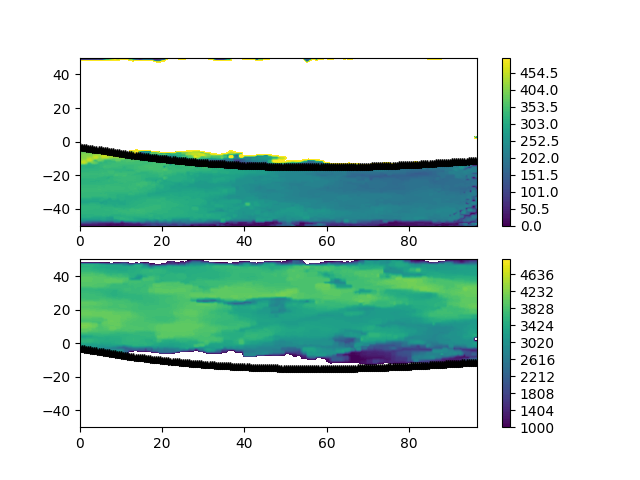
\includegraphics[scale=0.9]{oppg_b.png} 
\end{figure}

%C
\subsection{)}
\lstinputlisting{oppg_c.py}

funksjonen draw\_rects() bruker jeg i alle de neste oppgavene uten å definere eller importere funksjonen, ettersom alle opprinnelig lå i samme fil.

Pilene i væskefasen er så små at man ikke engang kan se retningen på de, men jeg føler at å lage et plot til med annerledes proposjoner bare vil være forvirrende(Hvertfall med de måtene jeg prøvde på..). Dette plottet viser at luften går mye fortere enn vannet, som er tilfellet.
\begin{figure}[h!]
        \centering 
        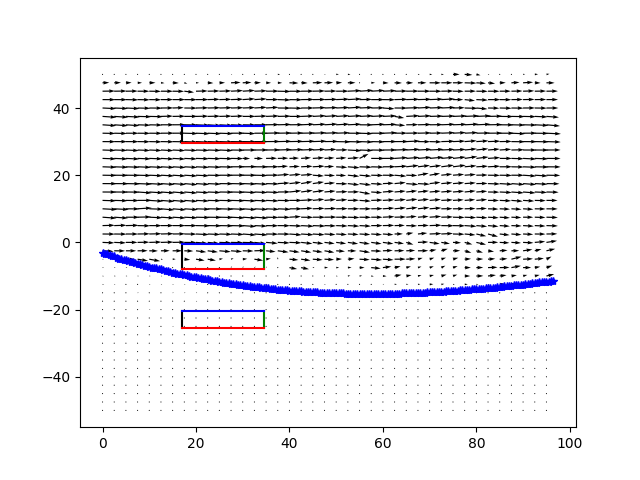
\includegraphics[scale=0.9]{oppg_c.png} 
\end{figure}

\pagebreak
%D
\subsection{)}
\lstinputlisting{oppg_d.py}

\begin{figure}[h!]
        \centering 
        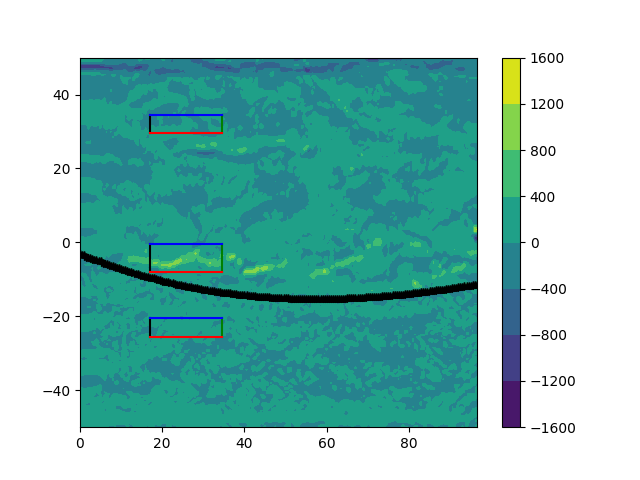
\includegraphics[scale=0.9]{oppg_d.png} 
\end{figure}
Divergensen til $u\vec{i} + v\vec{j}$ er ikke lik som divergensen til $v$ fordi den mangler w-komponenten. 
$v$ er definert ved $v = u\vec{i} + v\vec{j} + w\vec{k}$

Konsekvensen av at gassen og væsken er inkompressible er at divergensen til $v$ er 0. 
Dermed skjønner vi at w har verdier som cancele ut verdiene vi fikk for divergensen til $u\vec{i} + v\vec{j}$, ettersom divergensen til $u\vec{i} + v\vec{j} + w\vec{k}$ er 0


%E
\subsection{)}
\lstinputlisting{oppg_e.py}

\begin{figure}[h!]
        \centering 
        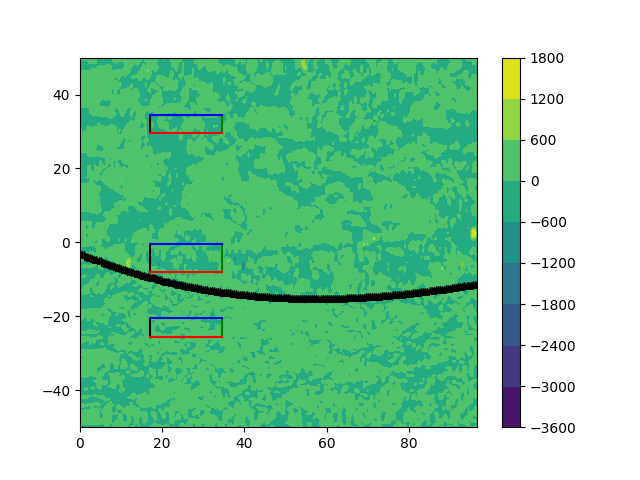
\includegraphics[scale=0.9]{oppg_e.png} 
\end{figure}

%F
\subsection{)}

Jeg får ikke samme resultat med flate- og kurveintegral.. Jeg tror det er flateintegralet som er feil, men får det ikke til.

\lstinputlisting{oppg_f.py}

\end{document}
